\clearpage\chapter{Unit Circle}
The unit circle is one of the most important concepts in pre-calculus (and this text). What you'll learn in this chapter you'll use for as long as you encounter trigonometric functions, which is a \textit{very} long time if you pursue mathematics.

After having covered special triangles in the previous chapter, we'll use them heavily when describing the unit circle. Don't worry if you haven't read that chapter. While it would help if you \textit{did} read it, you'll be able to follow along without it.

Unlike the special triangles, however, \textbf{I definitely recommend you understand what radians are and where they come from}. You can read the chapter on Radians in this text, or consult other resources available to you. Radians are crucial for describing the unit circle. The better your understanding of them, the easier the information in this chapter will come.

While you will eventually need to memorize and quickly recall the unit circle, I'll focus on the conceptual side of it. That is, I'll explain why the unit circle is constructed the way it is visually and algebraically. Only then will I continue to memorization.

This is probably the longest introduction to a chapter---I hope the rest of the it lives up to the hype.
\section{What Is The Unit Circle?}
The unit circle is a circle centered at the origin, $(0,0)$, with a radius of $1$ unit, hence the name "\textbf{unit} circle." Here it is:
\begin{center}
        \begin{minipage}[c]{0.45\linewidth}
                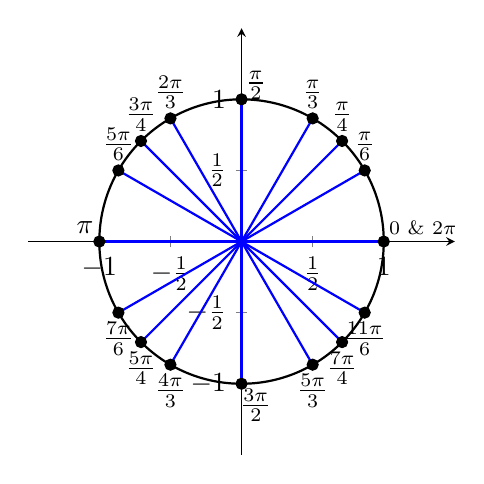
\begin{tikzpicture}
                        \begin{axis} [
                                xmin = -1.5, xmax = 1.5,
                                ymin = -1.5, ymax = 1.5,
                                height = 7cm, width = 7cm,
                                axis lines = middle,
                                xtick = {
                                -1, -0.5, 0, 0.5, 1
                                },
                                xticklabels = {
                                $-1$, $-\frac{1}{2}$, $0$, $\frac{1}{2}$, $1$%
                                },
                                ytick = {
                                -1, -0.5, 0, 0.5, 1
                                },
                                yticklabels = {
                                $-1$, $-\frac{1}{2}$, $0$, $\frac{1}{2}$, $1$%
                                }%
                        ]
                                \draw[color = black, thick] (0,0) circle (1); %Circle
                                \draw[color=blue, thick] ({-sqrt(3) / 2}, {-1/2}) -- ({sqrt(3) / 2}, {1/2}); % pi/6
                                \draw[color=blue, thick] ({-sqrt(3) / 2}, {1/2}) -- ({sqrt(3) / 2}, {-1/2}); % -pi/6
                                %
                                \draw[color=blue,thick] ({-sqrt(2)/2}, {-sqrt(2)/2}) -- ({sqrt(2)/2},{sqrt(2)/2}); % pi/4
                                \draw[color=blue,thick] ({-sqrt(2)/2},{sqrt(2)/2}) -- ({sqrt(2)/2},{-sqrt(2)/2}); % -pi/4
                                %
                                \draw[color=blue, thick] ({-1/2},{-sqrt(3) / 2}) -- ({1/2}, {sqrt(3) / 2}); % pi/3
                                \draw[color=blue, thick] ({-1/2}, {sqrt(3) / 2}) -- ({1/2}, {-sqrt(3) / 2}); % -pi/3
                                %
                                \draw[color=blue, thick] (0, -1) -- (0, 1);
                                \draw[color=blue,thick] (-1, 0) -- (1, 0);
                                %Quadrant I
                                \filldraw[black] ({sqrt(3) / 2}, {1/2}) circle (2pt) node[anchor=south] {$\frac{\pi}{6}$};
                                \filldraw[black] ({sqrt(2)/2},{sqrt(2)/2}) circle (2pt) node[anchor=south] {$\frac{\pi}{4}$};
                                \filldraw[black] ({1/2}, {sqrt(3) / 2}) circle (2pt) node[anchor=south] {$\frac{\pi}{3}$};
                                %Quadrant II
                                \filldraw[black] ({-sqrt(3) / 2}, {1/2}) circle (2pt) node[anchor=south] {$\frac{5\pi}{6}$};
                                \filldraw[black] ({-sqrt(2)/2},{sqrt(2)/2}) circle (2pt) node[anchor=south] {$\frac{3\pi}{4}$};
                                \filldraw[black] ({-1/2}, {sqrt(3) / 2}) circle (2pt) node[anchor=south] {$\frac{2\pi}{3}$};
                                %Quadrant III
                                \filldraw[black] ({-sqrt(3) / 2}, {-1/2}) circle (2pt) node[anchor=north] {$\frac{7\pi}{6}$};
                                \filldraw[black] ({-sqrt(2)/2},{-sqrt(2)/2}) circle (2pt) node[anchor=north] {$\frac{5\pi}{4}$};
                                \filldraw[black] ({-1/2}, {-sqrt(3) / 2}) circle (2pt) node[anchor=north] {$\frac{4\pi}{3}$};
                                %QUadrant IV
                                \filldraw[black] ({sqrt(3) / 2}, {-1/2}) circle (2pt) node[anchor=north] {$\frac{11\pi}{6}$};
                                \filldraw[black] ({sqrt(2)/2},{-sqrt(2)/2}) circle (2pt) node[anchor=north] {$\frac{7\pi}{4}$};
                                \filldraw[black] ({1/2}, {-sqrt(3) / 2}) circle (2pt) node[anchor=north] {$\frac{5\pi}{3}$};
                                %Points on Axis
                                \filldraw[black] (1,0) circle (2pt) node[font=\scriptsize] at (1.275,0.1) {$0$ \& $2\pi$};
                                \filldraw[black] (-1,0) circle (2pt) node at (-1.1,0.1) {$\pi$};
                                \filldraw[black] (0,1) circle (2pt) node at (0.1,1.1) {$\frac{\pi}{2}$};
                                \filldraw[black] (0,-1) circle (2pt) node at (0.1,-1.15) {$\frac{3\pi}{2}$};
                        \end{axis}
                \end{tikzpicture}
                \label{fig:UnitCircle}
        \end{minipage}
        \begin{minipage}[c]{0.54\linewidth}
                \begin{tabular}{ c | c | c | c }
                        Angle & Point & Angle & Point\\
                        \hline
                        $\frac{\pi}{6}$ & $\left(\frac{\sqrt{3}}{2}, \frac{1}{2} \right)$ 
                        & $\frac{7\pi}{6}$ & $\left(-\frac{\sqrt{3}}{2}, -\frac{1}{2} \right)$ \\
                        \hline
                        $\frac{\pi}{4}$ & $\left(\frac{\sqrt{2}}{2}, \frac{\sqrt{2}}{2} \right)$ 
                        & $\frac{5\pi}{4}$ & $\left(-\frac{\sqrt{2}}{2}, -\frac{\sqrt{2}}{2} \right)$ \\
                        \hline
                        $\frac{\pi}{3}$ & $\left(\frac{1}{2}, \frac{\sqrt{3}}{2} \right)$ 
                        & $\frac{4\pi}{3}$ & $\left(-\frac{1}{2}, -\frac{\sqrt{3}}{2} \right)$ \\
                        \hline
                        $\frac{\pi}{2}$ & $\left(0, 1 \right)$ 
                        & $\frac{3\pi}{2}$ & $\left(0, -1 \right)$ \\
                        \hline
                        $\frac{2\pi}{3}$ & $\left(-\frac{1}{2}, \frac{\sqrt{3}}{2} \right)$ 
                        & $\frac{5\pi}{3}$ & $\left(\frac{1}{2}, -\frac{\sqrt{3}}{2} \right)$ \\
                        \hline
                        $\frac{3\pi}{4}$ & $\left(-\frac{\sqrt{2}}{2}, \frac{\sqrt{2}}{2} \right)$ 
                        & $\frac{7\pi}{4}$ & $\left(\frac{\sqrt{2}}{2}, -\frac{\sqrt{2}}{2} \right)$ \\
                        \hline
                        $\frac{5\pi}{6}$ & $\left(-\frac{\sqrt{3}}{2}, \frac{1}{2} \right)$ 
                        & $\frac{11\pi}{6}$ & $\left(\frac{\sqrt{3}}{2}, -\frac{1}{2} \right)$ \\
                        \hline
                        $\pi$ & $\left(-1, 0 \right)$ & $0$ \& $2\pi$ 
                        & $\left(1, 0 \right)$ \\
                \end{tabular}
        \end{minipage}
\end{center}
The table at the right shows each of the values, in radians, with their corresponding $x$ and $y$ values.

If you draw a point directly to the $x$-axis line from each of the points, notice how you form right trangles with that line, the $x$-axis line itself, and the diagonal blue lines.